\documentclass[4pt,a4papper]{article}
\usepackage{ctex}  
\usepackage{amsmath}
\usepackage{mathtools}
\usepackage{upgreek}
\pagestyle{headings}
\usepackage{graphicx}
\usepackage{subfigure}
\usepackage{indentfirst}
\usepackage{fancyhdr}
\usepackage{listings}
\usepackage{amsmath}
\usepackage{longtable}
\usepackage{geometry}
\usepackage[usenames,dvipsnames]{color}
\definecolor{lightgray}{RGB}{230,230,230}
\lstset{ language=, numbers=left, basicstyle=\small,
  keywordstyle=\color{blue}, commentstyle=\color{PineGreen},
  stringstyle=\color{red}, frame=shadowbox, breaklines=true,
  backgroundcolor=\color{lightgray},extendedchars=false }


\geometry{left=1.5cm,right=1.5cm,top=3cm,bottom=1.5cm}

%opening
\title{\zihao{-2}\textbf{溶解焓实验报告}}
\author{张锦程}
\date{\today}

\begin{document}
\maketitle
%\tableofcontents

\section{\zihao{4}实验目的}
1.测量硝酸钾在不同浓度水溶液的溶解热,求硝酸钾在水中溶解过程的各种热效应。

2.掌握量热装置的基本组合及电热补偿法测定热效应的基本原理。

3.复习掌握常用的测温技术。 

\section{\zihao{4}实验原理}
物质溶于溶剂中,一般伴随有热效应的发生。盐类的溶解通常包含着几个同时进行的过程:晶格的破坏、离子或分子的溶剂化、分子电离(对电解质而言)等。热效应的大小和符号决定于溶剂及溶质的性质和它们的相对量。 

1.溶解热: 在恒温恒压下,溶质B溶于溶剂 A(或溶于某浓度溶液)中产生的热效应 $\Delta_{sol} H$

2.摩尔积分溶解热: $\Delta_sol H_m = \frac{\Delta_sol H}{n_B}$

3.摩尔微分溶解热: $(\frac{\partial \Delta_{sol}H}{\partial n_B})_{n_A}$

4.稀释热: 在恒温恒压下,一定量的溶剂 A 加到某浓度的溶液中使之稀释,所产生的热效应

5.摩尔积分稀释热: $\Delta_{dil}H_m = \Delta_{sol}H_{m_2} - \Delta_{sol}H_{m_1}$

6.摩尔微分稀释热: $(\frac{\partial \Delta_{sol}H}{\partial n_A})_{n_B}$

在恒温恒压下,对于指定的溶剂 A 和溶质 B,溶解热的大小取决于 A 和 B 的物质的量,即:  $\Delta_{sol}H = \int (n_A, n_B)$

可推导得:

$$\Delta_{sol}H_m=\frac{n_A}{n_B}(\frac{\partial \Delta_{sol}H}{\partial n_B})_{T,P,n_B} + (\frac{\partial \Delta_{sol}H}{\partial n_A})_{T,P,n_A}$$


令 $n_0 = \frac{n_A}{n_B}$ ,改写为:

$$\Delta_{sol}H_m=\frac{n_A}{n_B}(\frac{\partial \Delta_{sol}H}{\partial n_B})_{T,P,n_B} + (\frac{\partial \Delta_{sol}H}{\partial n_A})_{T,P,n_A}$$

式中的 $\Delta{sol}H_m$ 可由实验测定, $n_0$ 由实验中所用的溶质和溶剂的物质的量计算得到。作出曲线。切线的斜率为该浓度下的摩尔微分稀释热,切线与纵坐标的截距,为该浓度下的摩尔微分溶解热.

因本实验测定 $KNO_3$ 在水中的溶解热是一个吸热过程,热量的标定可用电热补偿法,即先测定体系的起始温度,溶解过程中体系温度随吸热反应进行而降低,再用电加热法使体系升温至起始温度,根据所消耗电能求出热效应 Q。再由下式可求算出溶解热:
$$\Delta_{sol}H = Q\frac{T_2 - T_1}{T_2^{/}-T_1^{/}}, Q=I^2RT$$

\section{\zihao{4}实验操作}
1.组装仪器,要求仪器装置绝热良好,体系和环境间的热交换尽量稳定并降至最小仪器装置如图 2-3-2 所示,采用保温瓶并加盖,以减少辐射、传导、对流、蒸发等热交换途径。 

2.测量室温,取不少于 500ml 的去离子水,根据室温调节水的温度,使之尽量接近室温,量取500ml注入保温瓶内。按图将装置安装好,记录仪量程 20mv,走纸速度 4mm/min。 

3.在天平上准确称量 5g 左右的 $KNO_3$ 粉末待用。

4、开动搅拌器,调节测温电桥平衡调节旋钮,使记录仪的记录笔处于记录纸的中间位置,待温度基本稳定后,记录约 4min(约记录纸的 1 格半)。直流稳压稳流电源调至稳流,打开电源开始加热,同时将电流值调至 950mA 左右(此后不要再调节电流),温度升高,记录笔升至约 70 格左右(记录纸上的刻度),关闭电源停止加热。待记录仪记录约 8min 左右,加入称量好的 $KNO_3$。此时由于 $KNO_3$ 溶解吸热,温度降低,记录笔降低,待温度稳定后再记录约 8min 左右。

5、打开加热电源加热,同时打开秒表计时,待记录笔升至 80 格左右(加热使温度升高的格数,以下次加入 $KNO_3$ 的量决定),关闭电源停止加热,同时停止计时,记下加热时间。再记录约 8min 左右。

6、按上述步骤依次加入约 6、7、8、8、7 和 6g 的 $KNO_3$。 

7、测量实验所用加热器的阻值 R


\section{\zihao{4}实验结果讨论}
\subsection{\zihao{-4}计算处理过程}
1.采用雷诺图解法,校正各步加热、溶解过程的峰高。

2.分别计算出各次加入样品 B 后的热效应,计算出摩尔积分溶解热 $\Delta_{sol}H_m$,并分别计算出对应的 $n_O = n_{H_2O}/n_B$。
3.将 $\Delta_{sol}H_m$ 与 $n_0$ 列表并作图。从图中分别求出 $n_0$ 为80、100、200、300、400 处的摩尔积分溶解热、微分溶解热、微分稀释热。再从图中求出为 80 → 100、100 → 200、200 → 300、300 → 400 过程的摩尔稀释热。

\subsection{\zihao{-4}测定结果}
首先根据雷洛修正法可作出下图的温度曲线:

    \begin{figure}[htbp]
        %\small
        \centering
        \includegraphics[width=20cm]{./figures/溶解焓数据处理.png}
        \caption{实验数据的雷洛图解法} \label{fig:1}
    \end{figure}
    \begin{figure}[htbp]
        %\small
        \centering
        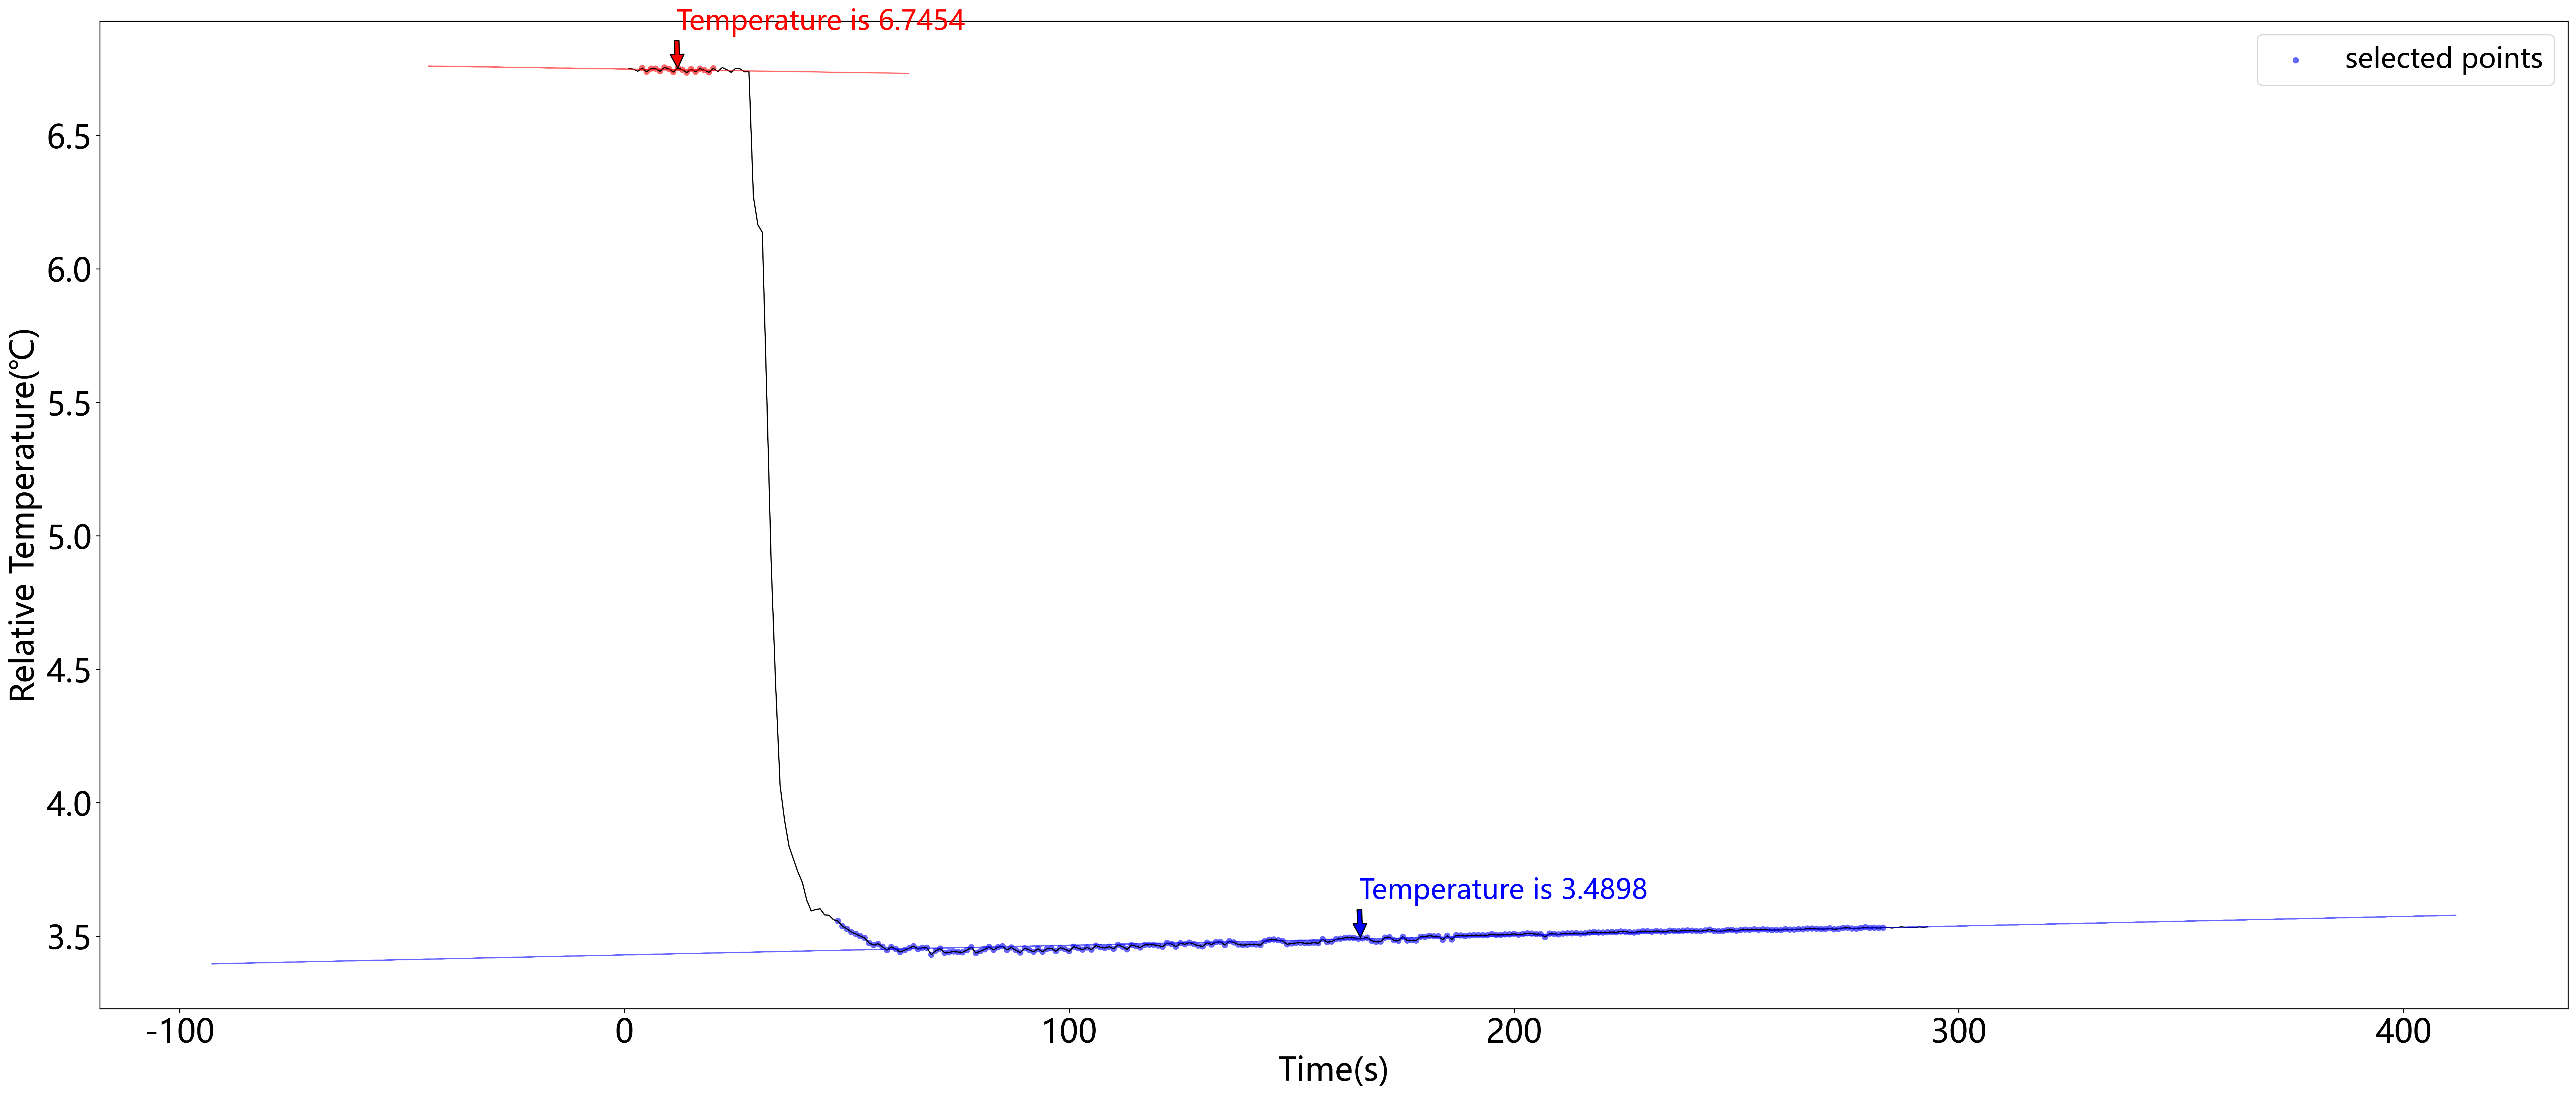
\includegraphics[width=14cm]{./figures/溶解焓数据处理-5.png}
        \caption{附图:加入 $5g\; KNO_3$时的降温曲线} \label{fig:1}
    \end{figure}


\subsection{\zihao{-4}讨论分析}
根据实验结果整理得下表:
\begin{table}[htbp]
\begin{tabular}{|c|c|c|c|c|c|c|c|}
\hline
组别         & 1       & 2           & 3           & 4           & 5          & 6           & 7           \\ \hline
电流(A)      & 0.95    & 0.95        & 0.95        & 0.95        & 0.95       & 0.95        & 0.95        \\ \hline
电阻(R)      & 16.39   & 16.39       & 16.39       & 16.39       & 16.39      & 16.39       & 16.39       \\ \hline
加热时间(s)    & 0       & 143.3666667 & 132.3166667 & 191.72      & 201.2      & 115.7833333 & 143.4166667 \\ \hline
电功(J)      & 0       & 2120.676149 & 1957.224825 & 2835.917447 & 2976.14537 & 1712.664172 & 2121.415748 \\ \hline
加热温度改变量(℃) & 0       & 4.3775      & 4.0663      & 5.8166      & 6.0808     & 3.5483      & 4.3428      \\ \hline
降温温度改变量(℃) & 3.2556  & 4.2547      & 4.7634      & 5.3428      & 5.2325     & 4.3104      & 3.6066      \\ \hline
加入硝酸钾质量(g) & 5. 0061 & 5.9971      & 6.917       & 8.0010      & 8.0012     & 6.9918      & 6.0011      \\ \hline
\end{tabular}
\end{table}

雷洛图解法要求每次升温后回到同一温度,但是观察图像可得这一要求并不满足,所以需要根据曲线来将每次加热所作电功数据转化为降温时 $K_NO_3$ 的溶解热数据。

具体操作上,我们可以近似将每次加热时的体系总热容 $C = \frac{dQ}{dT}$(非比热容)与紧邻的上一次降温时的系统比热容视作相等的,根据

$$\frac{Q_1}{Q_2} = \frac{T_1}{T_2}$$

求得修正后的结果:
\begin{table}[htbp]
\begin{tabular}{|c|c|c|c|c|c|c|c|}
\hline
组别                               & 1                            & 2                            & 3                            & 4                            & 5                            & 6                            & 7                            \\ \hline
硝酸钾质量 / g                        & 5. 0061                      & 5.9971                       & 6.917                        & 8.0010                       & 8.0012                       & 6.9918                       & 6.0011                       \\ \hline
\multicolumn{1}{|l|}{修正后溶解热 / J} & \multicolumn{1}{l|}{1577.17} & \multicolumn{1}{l|}{2047.90} & \multicolumn{1}{l|}{2322.42} & \multicolumn{1}{l|}{2614.94} & \multicolumn{1}{l|}{2525.58} & \multicolumn{1}{l|}{2105.59} & \multicolumn{1}{l|}{1761.79} \\ \hline
\end{tabular}
\end{table}

作图验证可得我们的修正是合理的
    \begin{figure}[htbp]
        %\small
        \centering
        \includegraphics[width=12cm]{./figures/溶解热 - 加入KNO_3质量2.png}
        \caption{修正后的溶解热 - 加入 $KNO_3$ 质量} \label{fig:2}
    \end{figure}

计算出 $\Delta_{sol}H_m$ 与对应的 $n_O = n_{H_2O}/n_B$ 见下:
\begin{table}[htbp]
\begin{tabular}{|l|l|l|l|l|l|l|l|}
\hline
\multicolumn{1}{|c|}{组别} & \multicolumn{1}{c|}{1} & \multicolumn{1}{c|}{2} & \multicolumn{1}{c|}{3} & \multicolumn{1}{c|}{4} & \multicolumn{1}{c|}{5} & \multicolumn{1}{c|}{6} & \multicolumn{1}{c|}{7} \\ \hline
$\Delta_{sol}H_m$ / J    & 1577.172               & 3625.079               & 5947.503               & 8562.446               & 11088.026              & 13193.615              & 14955.404              \\ \hline
n($KNO_3$) / mol         & 0.04951                & 0.108834               & 0.177252               & 0.256391               & 0.335533               & 0.404690               & 0.464048               \\ \hline
$n_O = n_{H_2O}/n_B$     & 560.5089496            & 255.0134372            & 156.5810567            & 108.2497667            & 82.71713831            & 68.58166242            & 59.80914228            \\ \hline
\end{tabular}
\end{table}

画出图像如下图所示:
    \begin{figure}[htbp]
        %\small
        \centering
        \includegraphics[width=16cm]{./figures/积分溶解热 - n_02.png}
        \caption{积分溶解热$\Delta_{sol}H_m$ - $n_0$} \label{fig:3}
    \end{figure}

最终的计算结果如下:
\begin{table}[htbp]
\begin{tabular}{|l|l|l|l|l|l|}
\hline
\multicolumn{1}{|c|}{组别} & \multicolumn{1}{c|}{1} & \multicolumn{1}{c|}{2} & \multicolumn{1}{c|}{3} & \multicolumn{1}{c|}{4} & \multicolumn{1}{c|}{5} \\ \hline
$n_O = n_{H_2O}/n_B$     & 80                     & 100                    & 200                    & 300                    & 400                    \\ \hline
$\Delta_{sol}H_m$ / J    & 11769.98554            & 9613.552874            & 4171.004503            & 2597.110803            & 2141.967144            \\ \hline
$\Delta_{dil}H_m$ / J    & -121.7516817           & -94.99693393           & -27.47151989           & -7.944302765           & -2.297359108           \\ \hline
\end{tabular}
\end{table}




\newpage


\section{\zihao{4}附录}
\subsection{\zihao{-4}思考题}
1.要做好这个实验关键因素有哪些?

(1)毛细管垂直放置,其端口要和液面刚好接触,同时保证固定毛细管和外接装置的气密性,若密封度低,则气泡 溢出段不稳定,而且测得压力偏低。 
(2)仔细调节抽气瓶的滴水速度,出泡速度不可太快,否则不能达到平衡。 
(3)溶液配制要准确,按浓度从低到高的顺序测量。 
(4)表面张力对温度敏感,每次都应将溶液在恒温槽中静置一段时间,恒温后再测量。 

2.气泡形成速度过快对结果有何影响? 

会。若形成速度太快则可能会难以在压差最大点保持平衡(气泡破裂)。另外气泡的形成的短暂时间内是一个非稳态的过程,形成速度过快则可能对周围溶液产生扰动。若形成速度适中则可以有充分的时间建立平衡。 

3.为什么毛细管端口要和液面刚好接触?毛细管内径均匀与否对结果有无影响? 

如果毛细管深入液面下方太多,则测出的压差就包括了液面下方高度所产生的水压,导致了实验的误差。 无影响。实际上毛细管主体部分没有太大作用,主要起作用的是毛细管尖部分,主要应该保证端口处平整、半径均匀即可。


\clearpage
\end{document}